\documentclass[twoside]{book}

% Packages required by doxygen
\usepackage{fixltx2e}
\usepackage{calc}
\usepackage{doxygen}
\usepackage[export]{adjustbox} % also loads graphicx
\usepackage{graphicx}
\usepackage[utf8]{inputenc}
\usepackage{makeidx}
\usepackage{multicol}
\usepackage{multirow}
\PassOptionsToPackage{warn}{textcomp}
\usepackage{textcomp}
\usepackage[nointegrals]{wasysym}
\usepackage[table]{xcolor}

% Font selection
\usepackage[T1]{fontenc}
\usepackage[scaled=.90]{helvet}
\usepackage{courier}
\usepackage{amssymb}
\usepackage{sectsty}
\renewcommand{\familydefault}{\sfdefault}
\allsectionsfont{%
  \fontseries{bc}\selectfont%
  \color{darkgray}%
}
\renewcommand{\DoxyLabelFont}{%
  \fontseries{bc}\selectfont%
  \color{darkgray}%
}
\newcommand{\+}{\discretionary{\mbox{\scriptsize$\hookleftarrow$}}{}{}}

% Page & text layout
\usepackage{geometry}
\geometry{%
  a4paper,%
  top=2.5cm,%
  bottom=2.5cm,%
  left=2.5cm,%
  right=2.5cm%
}
\tolerance=750
\hfuzz=15pt
\hbadness=750
\setlength{\emergencystretch}{15pt}
\setlength{\parindent}{0cm}
\setlength{\parskip}{3ex plus 2ex minus 2ex}
\makeatletter
\renewcommand{\paragraph}{%
  \@startsection{paragraph}{4}{0ex}{-1.0ex}{1.0ex}{%
    \normalfont\normalsize\bfseries\SS@parafont%
  }%
}
\renewcommand{\subparagraph}{%
  \@startsection{subparagraph}{5}{0ex}{-1.0ex}{1.0ex}{%
    \normalfont\normalsize\bfseries\SS@subparafont%
  }%
}
\makeatother

% Headers & footers
\usepackage{fancyhdr}
\pagestyle{fancyplain}
\fancyhead[LE]{\fancyplain{}{\bfseries\thepage}}
\fancyhead[CE]{\fancyplain{}{}}
\fancyhead[RE]{\fancyplain{}{\bfseries\leftmark}}
\fancyhead[LO]{\fancyplain{}{\bfseries\rightmark}}
\fancyhead[CO]{\fancyplain{}{}}
\fancyhead[RO]{\fancyplain{}{\bfseries\thepage}}
\fancyfoot[LE]{\fancyplain{}{}}
\fancyfoot[CE]{\fancyplain{}{}}
\fancyfoot[RE]{\fancyplain{}{\bfseries\scriptsize Generated by Doxygen }}
\fancyfoot[LO]{\fancyplain{}{\bfseries\scriptsize Generated by Doxygen }}
\fancyfoot[CO]{\fancyplain{}{}}
\fancyfoot[RO]{\fancyplain{}{}}
\renewcommand{\footrulewidth}{0.4pt}
\renewcommand{\chaptermark}[1]{%
  \markboth{#1}{}%
}
\renewcommand{\sectionmark}[1]{%
  \markright{\thesection\ #1}%
}

% Indices & bibliography
\usepackage{natbib}
\usepackage[titles]{tocloft}
\setcounter{tocdepth}{3}
\setcounter{secnumdepth}{5}
\makeindex

% Hyperlinks (required, but should be loaded last)
\usepackage{ifpdf}
\ifpdf
  \usepackage[pdftex,pagebackref=true]{hyperref}
\else
  \usepackage[ps2pdf,pagebackref=true]{hyperref}
\fi
\hypersetup{%
  colorlinks=true,%
  linkcolor=blue,%
  citecolor=blue,%
  unicode%
}

% Custom commands
\newcommand{\clearemptydoublepage}{%
  \newpage{\pagestyle{empty}\cleardoublepage}%
}

\usepackage{caption}
\captionsetup{labelsep=space,justification=centering,font={bf},singlelinecheck=off,skip=4pt,position=top}

%===== C O N T E N T S =====

\begin{document}

% Titlepage & ToC
\hypersetup{pageanchor=false,
             bookmarksnumbered=true,
             pdfencoding=unicode
            }
\pagenumbering{alph}
\begin{titlepage}
\vspace*{7cm}
\begin{center}%
{\Large D\+R\+E\+SS }\\
\vspace*{1cm}
{\large Generated by Doxygen 1.8.13}\\
\end{center}
\end{titlepage}
\clearemptydoublepage
\pagenumbering{roman}
\tableofcontents
\clearemptydoublepage
\pagenumbering{arabic}
\hypersetup{pageanchor=true}

%--- Begin generated contents ---
\chapter{Class Index}
\section{Class List}
Here are the classes, structs, unions and interfaces with brief descriptions\+:\begin{DoxyCompactList}
\item\contentsline{section}{\hyperlink{classWebServer}{Web\+Server} \\*The \hyperlink{classWebServer}{Web\+Server} class }{\pageref{classWebServer}}{}
\end{DoxyCompactList}

\chapter{File Index}
\section{File List}
Here is a list of all files with brief descriptions\+:\begin{DoxyCompactList}
\item\contentsline{section}{G\+U\+I/\hyperlink{main_8cpp}{main.\+cpp} }{\pageref{main_8cpp}}{}
\item\contentsline{section}{G\+U\+I/\hyperlink{WebServer_8cpp}{Web\+Server.\+cpp} }{\pageref{WebServer_8cpp}}{}
\item\contentsline{section}{G\+U\+I/\hyperlink{WebServer_8h}{Web\+Server.\+h} }{\pageref{WebServer_8h}}{}
\end{DoxyCompactList}

\chapter{Class Documentation}
\hypertarget{classWebServer}{}\section{Web\+Server Class Reference}
\label{classWebServer}\index{Web\+Server@{Web\+Server}}


The \hyperlink{classWebServer}{Web\+Server} class.  




{\ttfamily \#include $<$Web\+Server.\+h$>$}

\subsection*{Public Types}
\begin{DoxyCompactItemize}
\item 
enum \hyperlink{classWebServer_a350f14f5d1522610502fb95f346e4a3c}{Status} \+: uint8\+\_\+t \{ \newline
\hyperlink{classWebServer_a350f14f5d1522610502fb95f346e4a3ca1d451f0e2a986b2d755301fc16327831}{U\+N\+K\+N\+O\+WN} = 0, 
\hyperlink{classWebServer_a350f14f5d1522610502fb95f346e4a3ca8dd909a7ebd4b0b25ef0af0c754deb53}{S\+T\+O\+P\+P\+ED} = 1, 
\hyperlink{classWebServer_a350f14f5d1522610502fb95f346e4a3caf0cc930cb72ab6a5d0bca765bab81c19}{R\+U\+N\+N\+I\+NG} = 2, 
\hyperlink{classWebServer_a350f14f5d1522610502fb95f346e4a3ca229029746647a912e8c8f8366f2efacb}{S\+T\+A\+R\+T\+I\+NG} = 3, 
\newline
\hyperlink{classWebServer_a350f14f5d1522610502fb95f346e4a3ca46f07f457962a112a550b7b69a7dcdb8}{S\+T\+O\+P\+P\+I\+NG} = 4, 
\hyperlink{classWebServer_a350f14f5d1522610502fb95f346e4a3ca2187c4c7fce9bed9a2f66b8e835676e7}{E\+R\+R\+OR} = 5
 \}\begin{DoxyCompactList}\small\item\em The Status enum Lists the possible states the \hyperlink{classWebServer}{Web\+Server} may take. \end{DoxyCompactList}
\end{DoxyCompactItemize}
\subsection*{Public Member Functions}
\begin{DoxyCompactItemize}
\item 
\hyperlink{classWebServer_a456687b9d497b2810e3660f08bfa8462}{Web\+Server} (uint32\+\_\+t port=80)
\begin{DoxyCompactList}\small\item\em \hyperlink{classWebServer}{Web\+Server}. \end{DoxyCompactList}\item 
bool \hyperlink{classWebServer_a0ce9a771f7adb84c47c748a9a19444fe}{Start} ()
\begin{DoxyCompactList}\small\item\em Start. \end{DoxyCompactList}\item 
bool \hyperlink{classWebServer_af27f38bac6c5f718ae25deeb3369fb8a}{Stop} ()
\begin{DoxyCompactList}\small\item\em Stop. \end{DoxyCompactList}\item 
\hyperlink{classWebServer_a350f14f5d1522610502fb95f346e4a3c}{Status} \hyperlink{classWebServer_a191564ab545bdb1aa90ed40cfa966836}{Get\+Status} ()
\begin{DoxyCompactList}\small\item\em Get\+Status. \end{DoxyCompactList}\end{DoxyCompactItemize}
\subsection*{Private Attributes}
\begin{DoxyCompactItemize}
\item 
\hyperlink{classWebServer_a350f14f5d1522610502fb95f346e4a3c}{Status} \hyperlink{classWebServer_acde07bc97f932a6690ab659625309562}{\+\_\+status}
\end{DoxyCompactItemize}


\subsection{Detailed Description}
The \hyperlink{classWebServer}{Web\+Server} class. 


\begin{DoxyImageNoCaption}
  \mbox{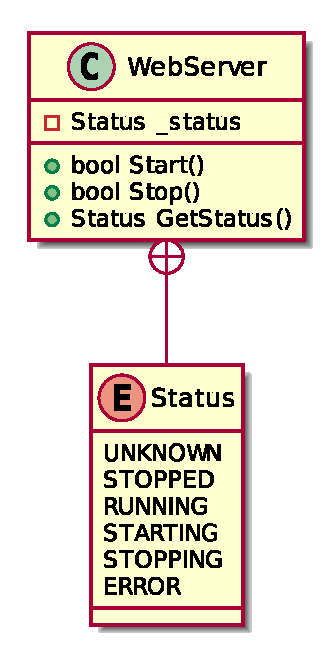
\includegraphics[width=\textwidth,height=\textheight/2,keepaspectratio=true]{inline_umlgraph_2}}
\end{DoxyImageNoCaption}
 

\subsection{Member Enumeration Documentation}
\mbox{\Hypertarget{classWebServer_a350f14f5d1522610502fb95f346e4a3c}\label{classWebServer_a350f14f5d1522610502fb95f346e4a3c}} 
\index{Web\+Server@{Web\+Server}!Status@{Status}}
\index{Status@{Status}!Web\+Server@{Web\+Server}}
\subsubsection{\texorpdfstring{Status}{Status}}
{\footnotesize\ttfamily enum \hyperlink{classWebServer_a350f14f5d1522610502fb95f346e4a3c}{Web\+Server\+::\+Status} \+: uint8\+\_\+t}



The Status enum Lists the possible states the \hyperlink{classWebServer}{Web\+Server} may take. 

\begin{DoxyEnumFields}{Enumerator}
\raisebox{\heightof{T}}[0pt][0pt]{\index{U\+N\+K\+N\+O\+WN@{U\+N\+K\+N\+O\+WN}!Web\+Server@{Web\+Server}}\index{Web\+Server@{Web\+Server}!U\+N\+K\+N\+O\+WN@{U\+N\+K\+N\+O\+WN}}}\mbox{\Hypertarget{classWebServer_a350f14f5d1522610502fb95f346e4a3ca1d451f0e2a986b2d755301fc16327831}\label{classWebServer_a350f14f5d1522610502fb95f346e4a3ca1d451f0e2a986b2d755301fc16327831}} 
U\+N\+K\+N\+O\+WN&\\
\hline

\raisebox{\heightof{T}}[0pt][0pt]{\index{S\+T\+O\+P\+P\+ED@{S\+T\+O\+P\+P\+ED}!Web\+Server@{Web\+Server}}\index{Web\+Server@{Web\+Server}!S\+T\+O\+P\+P\+ED@{S\+T\+O\+P\+P\+ED}}}\mbox{\Hypertarget{classWebServer_a350f14f5d1522610502fb95f346e4a3ca8dd909a7ebd4b0b25ef0af0c754deb53}\label{classWebServer_a350f14f5d1522610502fb95f346e4a3ca8dd909a7ebd4b0b25ef0af0c754deb53}} 
S\+T\+O\+P\+P\+ED&\\
\hline

\raisebox{\heightof{T}}[0pt][0pt]{\index{R\+U\+N\+N\+I\+NG@{R\+U\+N\+N\+I\+NG}!Web\+Server@{Web\+Server}}\index{Web\+Server@{Web\+Server}!R\+U\+N\+N\+I\+NG@{R\+U\+N\+N\+I\+NG}}}\mbox{\Hypertarget{classWebServer_a350f14f5d1522610502fb95f346e4a3caf0cc930cb72ab6a5d0bca765bab81c19}\label{classWebServer_a350f14f5d1522610502fb95f346e4a3caf0cc930cb72ab6a5d0bca765bab81c19}} 
R\+U\+N\+N\+I\+NG&\\
\hline

\raisebox{\heightof{T}}[0pt][0pt]{\index{S\+T\+A\+R\+T\+I\+NG@{S\+T\+A\+R\+T\+I\+NG}!Web\+Server@{Web\+Server}}\index{Web\+Server@{Web\+Server}!S\+T\+A\+R\+T\+I\+NG@{S\+T\+A\+R\+T\+I\+NG}}}\mbox{\Hypertarget{classWebServer_a350f14f5d1522610502fb95f346e4a3ca229029746647a912e8c8f8366f2efacb}\label{classWebServer_a350f14f5d1522610502fb95f346e4a3ca229029746647a912e8c8f8366f2efacb}} 
S\+T\+A\+R\+T\+I\+NG&\\
\hline

\raisebox{\heightof{T}}[0pt][0pt]{\index{S\+T\+O\+P\+P\+I\+NG@{S\+T\+O\+P\+P\+I\+NG}!Web\+Server@{Web\+Server}}\index{Web\+Server@{Web\+Server}!S\+T\+O\+P\+P\+I\+NG@{S\+T\+O\+P\+P\+I\+NG}}}\mbox{\Hypertarget{classWebServer_a350f14f5d1522610502fb95f346e4a3ca46f07f457962a112a550b7b69a7dcdb8}\label{classWebServer_a350f14f5d1522610502fb95f346e4a3ca46f07f457962a112a550b7b69a7dcdb8}} 
S\+T\+O\+P\+P\+I\+NG&\\
\hline

\raisebox{\heightof{T}}[0pt][0pt]{\index{E\+R\+R\+OR@{E\+R\+R\+OR}!Web\+Server@{Web\+Server}}\index{Web\+Server@{Web\+Server}!E\+R\+R\+OR@{E\+R\+R\+OR}}}\mbox{\Hypertarget{classWebServer_a350f14f5d1522610502fb95f346e4a3ca2187c4c7fce9bed9a2f66b8e835676e7}\label{classWebServer_a350f14f5d1522610502fb95f346e4a3ca2187c4c7fce9bed9a2f66b8e835676e7}} 
E\+R\+R\+OR&\\
\hline

\end{DoxyEnumFields}


\subsection{Constructor \& Destructor Documentation}
\mbox{\Hypertarget{classWebServer_a456687b9d497b2810e3660f08bfa8462}\label{classWebServer_a456687b9d497b2810e3660f08bfa8462}} 
\index{Web\+Server@{Web\+Server}!Web\+Server@{Web\+Server}}
\index{Web\+Server@{Web\+Server}!Web\+Server@{Web\+Server}}
\subsubsection{\texorpdfstring{Web\+Server()}{WebServer()}}
{\footnotesize\ttfamily Web\+Server\+::\+Web\+Server (\begin{DoxyParamCaption}\item[{uint32\+\_\+t}]{port = {\ttfamily 80} }\end{DoxyParamCaption})}



\hyperlink{classWebServer}{Web\+Server}. 


\begin{DoxyParams}{Parameters}
{\em port} & Optional parameter to specify a non-\/standard port for the server \\
\hline
\end{DoxyParams}


\subsection{Member Function Documentation}
\mbox{\Hypertarget{classWebServer_a191564ab545bdb1aa90ed40cfa966836}\label{classWebServer_a191564ab545bdb1aa90ed40cfa966836}} 
\index{Web\+Server@{Web\+Server}!Get\+Status@{Get\+Status}}
\index{Get\+Status@{Get\+Status}!Web\+Server@{Web\+Server}}
\subsubsection{\texorpdfstring{Get\+Status()}{GetStatus()}}
{\footnotesize\ttfamily \hyperlink{classWebServer_a350f14f5d1522610502fb95f346e4a3c}{Status} Web\+Server\+::\+Get\+Status (\begin{DoxyParamCaption}{ }\end{DoxyParamCaption})}



Get\+Status. 

\begin{DoxyReturn}{Returns}
A Status value which indicates the {\ttfamily \hyperlink{classWebServer}{Web\+Server}\textquotesingle{}s} current status. 
\end{DoxyReturn}
\mbox{\Hypertarget{classWebServer_a0ce9a771f7adb84c47c748a9a19444fe}\label{classWebServer_a0ce9a771f7adb84c47c748a9a19444fe}} 
\index{Web\+Server@{Web\+Server}!Start@{Start}}
\index{Start@{Start}!Web\+Server@{Web\+Server}}
\subsubsection{\texorpdfstring{Start()}{Start()}}
{\footnotesize\ttfamily bool Web\+Server\+::\+Start (\begin{DoxyParamCaption}{ }\end{DoxyParamCaption})}



Start. 

\begin{DoxyReturn}{Returns}
True if the server was successfully started. Otherwise false. 
\end{DoxyReturn}
\mbox{\Hypertarget{classWebServer_af27f38bac6c5f718ae25deeb3369fb8a}\label{classWebServer_af27f38bac6c5f718ae25deeb3369fb8a}} 
\index{Web\+Server@{Web\+Server}!Stop@{Stop}}
\index{Stop@{Stop}!Web\+Server@{Web\+Server}}
\subsubsection{\texorpdfstring{Stop()}{Stop()}}
{\footnotesize\ttfamily bool Web\+Server\+::\+Stop (\begin{DoxyParamCaption}{ }\end{DoxyParamCaption})}



Stop. 

\begin{DoxyReturn}{Returns}
True if the server was successfully stopped. Otherwise false. 
\end{DoxyReturn}


\subsection{Member Data Documentation}
\mbox{\Hypertarget{classWebServer_acde07bc97f932a6690ab659625309562}\label{classWebServer_acde07bc97f932a6690ab659625309562}} 
\index{Web\+Server@{Web\+Server}!\+\_\+status@{\+\_\+status}}
\index{\+\_\+status@{\+\_\+status}!Web\+Server@{Web\+Server}}
\subsubsection{\texorpdfstring{\+\_\+status}{\_status}}
{\footnotesize\ttfamily \hyperlink{classWebServer_a350f14f5d1522610502fb95f346e4a3c}{Status} Web\+Server\+::\+\_\+status\hspace{0.3cm}{\ttfamily [private]}}



The documentation for this class was generated from the following files\+:\begin{DoxyCompactItemize}
\item 
G\+U\+I/\hyperlink{WebServer_8h}{Web\+Server.\+h}\item 
G\+U\+I/\hyperlink{WebServer_8cpp}{Web\+Server.\+cpp}\end{DoxyCompactItemize}

\chapter{File Documentation}
\hypertarget{main_8cpp}{}\section{G\+U\+I/main.cpp File Reference}
\label{main_8cpp}\index{G\+U\+I/main.\+cpp@{G\+U\+I/main.\+cpp}}
{\ttfamily \#include $<$iostream$>$}\newline
Include dependency graph for main.\+cpp\+:\nopagebreak
\begin{figure}[H]
\begin{center}
\leavevmode
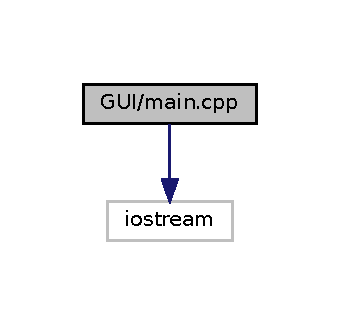
\includegraphics[width=163pt]{main_8cpp__incl}
\end{center}
\end{figure}
\subsection*{Functions}
\begin{DoxyCompactItemize}
\item 
int \hyperlink{main_8cpp_ae66f6b31b5ad750f1fe042a706a4e3d4}{main} ()
\end{DoxyCompactItemize}


\subsection{Function Documentation}
\mbox{\Hypertarget{main_8cpp_ae66f6b31b5ad750f1fe042a706a4e3d4}\label{main_8cpp_ae66f6b31b5ad750f1fe042a706a4e3d4}} 
\index{main.\+cpp@{main.\+cpp}!main@{main}}
\index{main@{main}!main.\+cpp@{main.\+cpp}}
\subsubsection{\texorpdfstring{main()}{main()}}
{\footnotesize\ttfamily int main (\begin{DoxyParamCaption}{ }\end{DoxyParamCaption})}


\hypertarget{WebServer_8cpp}{}\section{G\+U\+I/\+Web\+Server.cpp File Reference}
\label{WebServer_8cpp}\index{G\+U\+I/\+Web\+Server.\+cpp@{G\+U\+I/\+Web\+Server.\+cpp}}
{\ttfamily \#include \char`\"{}Web\+Server.\+h\char`\"{}}\newline
Include dependency graph for Web\+Server.\+cpp\+:\nopagebreak
\begin{figure}[H]
\begin{center}
\leavevmode
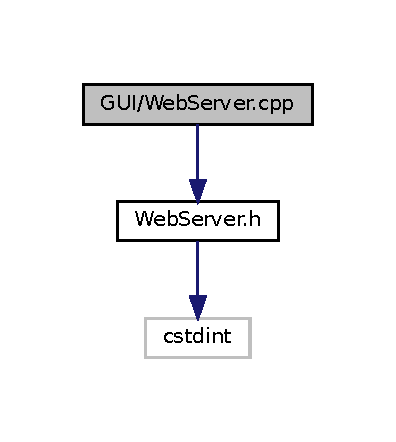
\includegraphics[width=190pt]{WebServer_8cpp__incl}
\end{center}
\end{figure}

\hypertarget{WebServer_8h}{}\section{G\+U\+I/\+Web\+Server.h File Reference}
\label{WebServer_8h}\index{G\+U\+I/\+Web\+Server.\+h@{G\+U\+I/\+Web\+Server.\+h}}
{\ttfamily \#include $<$cstdint$>$}\newline
Include dependency graph for Web\+Server.\+h\+:\nopagebreak
\begin{figure}[H]
\begin{center}
\leavevmode
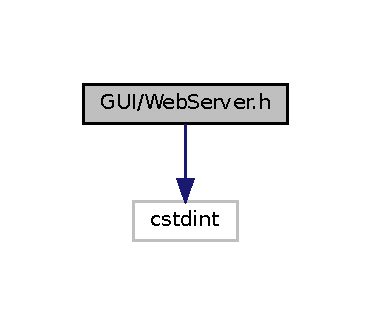
\includegraphics[width=178pt]{WebServer_8h__incl}
\end{center}
\end{figure}
This graph shows which files directly or indirectly include this file\+:\nopagebreak
\begin{figure}[H]
\begin{center}
\leavevmode
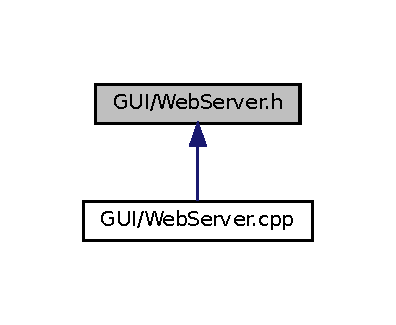
\includegraphics[width=190pt]{WebServer_8h__dep__incl}
\end{center}
\end{figure}
\subsection*{Classes}
\begin{DoxyCompactItemize}
\item 
class \hyperlink{classWebServer}{Web\+Server}
\begin{DoxyCompactList}\small\item\em The \hyperlink{classWebServer}{Web\+Server} class. \end{DoxyCompactList}\end{DoxyCompactItemize}

%--- End generated contents ---

% Index
\backmatter
\newpage
\phantomsection
\clearemptydoublepage
\addcontentsline{toc}{chapter}{Index}
\printindex

\end{document}
